\documentclass[a4paper,12pt]{article} % тип документа

% Поля страниц
\usepackage[left=2.5cm,right=2.5cm,
    top=2cm,bottom=2cm,bindingoffset=0cm]{geometry}
    
%Пакет дял таблиц   
\usepackage{multirow} 
    
%Отступ после заголовка    
\usepackage{indentfirst}


% Рисунки
\usepackage{floatrow,graphicx,calc}
\usepackage{wrapfig}

% Создаёем новый разделитель
\DeclareFloatSeparators{mysep}{\hspace{1cm}}

% Ссылки?
\usepackage{hyperref}
\usepackage[rgb]{xcolor}
\hypersetup{				% Гиперссылки
    colorlinks=true,       	% false: ссылки в рамках
	urlcolor=blue          % на URL
}


%  Русский язык
\usepackage[T2A]{fontenc}			% кодировка
\usepackage[utf8]{inputenc}			% кодировка исходного текста
\usepackage[english,russian]{babel}	% локализация и переносы


% Математика
\usepackage{amsmath,amsfonts,amssymb,amsthm,mathtools}


% Что-то 
\usepackage{wasysym}


%Заговолок
\author{Серебренников Даниил Б02-826}
\title{Лабораторная работа \No 2.1.5}


\begin{document}


\begin{center}
\footnotesize{ФЕДЕРАЛЬНОЕ ГОСУДАРСТВЕННОЕ АВТОНОМНОЕ ОБРАЗОВАТЕЛЬНОЕ 			УЧРЕЖДЕНИЕ ВЫСШЕГО ОБРАЗОВАНИЯ}\\
\footnotesize{МОСКОВСКИЙ ФИЗИКО-ТЕХНИЧЕСКИЙ ИНСТИТУТ\\(НАЦИОНАЛЬНЫЙ 			ИССЛЕДОВАТЕЛЬСКИЙ УНИВЕРСИТЕТ)}\\
\footnotesize{ФАКУЛЬТЕТ ОБЩЕЙ И ПРИКЛАДНОЙ ФИЗИКИ\\}
\hfill \break
\hfill\break
\hfill\break
\hfill \break
\hfill \break
\hfill \break
\hfill \break
\hfill \break
\hfill \break
\hfill \break
\hfill \break
\hfill \break
\hfill \break
\hfill \break
\large{Лабораторная работа № 2.1.5\\\textbf{Исследование термических эффектов, позникающих при упругих деформациях}}\\
\hfill \break
\hfill \break
\hfill \break
\begin{flushright}
	Серебренников Даниил\\
	Группа Б02-826
\end{flushright}
\hfill \break
\hfill \break
\hfill \break
\hfill \break
\hfill \break
\end{center}
\hfill \break
\hfill \break
\hfill \break
\hfill \break
\hfill \break
\hfill \break
\begin{center}
	Долгопрудный, 2019 г.
\end{center}
\thispagestyle{empty} % выключаем отображение номера для этой страницы


\newpage
	\textbf{Цель работы:} 1) исследование упругого деформирования резиновой пленки, в том числе при при больших удлининениях, когда оно становистя нелинейным; 2) измерение нагревания пленки при большом адибатчиеском растяжении и опредление теплоемкости пленки.
	
	\textbf{В работе используются:} образец резины, закрпленный в специальной установке; набор грузов; дифференциальная термопара; осциллограф <<GDS-71054B>>.
	
\section{Теоретическая часть}
	\subsection{Природа нагревания резины при растяжении}
		Нагревание резин при растяжении можно понять, рассматривая их молекулярную структуру. Полимерные молекулы, из которых состоит резина, представляют собой длинные цепи углеродных (или кремниевых) атомов, нерегулярным образом свернутые в клубки. Такие «макромолекулы» случайными химическими связями соединены с соседними молекулами. Образование «сшивок» происходит в процессе вулканизации резин; чем их больше, тем резина жестче.

		«Макромолекулы» участвуют в тепловом движении, практически независимо друг от друга при отсутствии растяжения, и на каждую из них приходится тепловая энергия в соответствии с числом степеней свободы. Но при растяжении резины «макромолекулы» уже не могут двигаться независимо друг от друга, так как растягивающие силы объединяют их в более жесткое образование, более жесткую молекулу. Поэтому часть степеней свободы клубков «замораживается». При этом некоторая доля тепловой энергии клубков переходит в тепловую энергию молекулы и температура резины по этой причине может расти.
	
		Тот же результат можно получить и из термодинамических соображений. При растяжении резины происходит частичная ориентация клубков макромолекул, т. е. полный «беспорядок» в молекулярной структуре полимера сменяется частичным порядком. Упорядочение межмолекулярной структуры эквивалентно уменьшению энтропии образца (напомним, что в кинетической теории энтропия характеризует степень беспорядка в физической системе). Так как полная энтропия образца в условиях нашего эксперимента должна оставаться постоянной, ориентационное уменьшение энтропии должно компенсироваться усилением хаотического движения различных частей молекул друг относительно друга, иначе говоря, повышением температуры образца.
	
	\subsection{Формальное описание нагревания резины}
		Вместо того, чтобы исследовать поглощение или выделение тепла при изотермическом процессе, можно изучать изменение температуры теплоизолированного тела. Если процесс происходит быстро, то тело можно не изолировать, поскольку процессы теплообмена идут медленно. В этом случае речь идёт об изоэнтропийном расстяжении образца. Поэтому в нашем случае связь между удлинением образца и изменением его температуры может быть выражена следующей формулой
			\begin{equation} \label{eq:dT}
				dT = \frac{T}{C_l}\biggr(\frac{\partial f}{\partial T}\biggl)_l dl,
			\end{equation}
где $C_l$ - теплоемкость образца при постоянной длине. При больших изменениях длины образца выражение~(\ref{eq:dT}) следует проинтегрировать. Изменения температуры обычной невелики, поэтому можно заменить $T$ на $T_0$:
			\begin{equation} \label{eq:S_dT}
				T - T_0 = \frac{T_0}{C_l} \int\limits_{l_0}^l \biggr(\frac{\partial f}{\partial T}\biggl)_l\,dl.
			\end{equation}
Формула~(\ref{eq:S_dT}) является окончательной и может быть применена для расчетов, если известна зависимость $f$ от $l$ и $T$. Эта зависимость не может быть поулчена теоретически и берется из опыта.
		
		У каучуков и резины модуль Юнга зависит как от удлинения, так и от температуры. Связь между $f$, $l$ и $T$ может быть описана эмпирической формулой
			\begin{equation} \label{eq:f=f(l,T)}
				f = \frac{E(T)\sigma_0}{3}\biggr[\lambda - \frac{1 + 3\alpha (T - T_0)}{\lambda^2}\biggl]
			\end{equation}
Здесь $\lambda = l / l_0$, а $\sigma_0$ - начальное поперечное сечение образца. Модуль Юнга у резины пропорционален T:
			\begin{equation} \label{eq:E=E(T)}
				E = \varkappa T.
			\end{equation}
		Для вычисления термического эффекта при расстяжении резинового образца подставим (\ref{eq:f=f(l,T)}) и (\ref{eq:E=E(T)}) в (\ref{eq:S_dT}). Интегрирование даёт
			\begin{equation} \label{eq:DT}
				\Delta T = T - T_0 = \frac{E \sigma_0 l_0}{6C_l} (\lambda - 1) \biggr[\lambda + 1 - \frac{2}{\lambda} (1 + 3\alpha T_0) \biggl].
			\end{equation}				
		Нетрудно видеть, что при увеличении $\lambda$ температура образца сначала уменьшается, а потом увеличивается. Пока $\lambda$ мало отличается от единицы, естественно положить $\lambda = 1 + \Delta l/l$. Квадратная скобка в правой части~(\ref{eq:DT}) при этом равна
			\begin{equation*}
				3\biggr( \frac{\Delta l}{l} - 2\alpha T_0 \biggl).
			\end{equation*}
		При совсем малых $\Delta l / l$ в этом выражении основную роль играет второй член, так что температура при растяжении падает. Это вполне естественно, так как небольшие растяжения резины хорошо описываются обычным законом Гука.

\section{Экспериментальная установка}
	Схема установки приведена на рис.~\ref{ris:ustanovka} Исследуемый образец резины 1 расположен внутри кожуха из оргстекла 2 и закреплен по торцам в двух зажимах 3, 11. Верхний зажим неподвижен, а нижний может перемещаться вдоль двух верти- кальных направляющих 4. Положение нижнего зажима определяется с помощью линейки 10, размещенной позади него. К подвижному зажиму 3 подвешена легкая платформа 5, расположенная снаружи кожуха. Резина растягивается грузом Р, помещаемым на платформу. Растяжение образца может быть ограничено положением упора 7, фиксируемого винтами 6, 9 на стойках 8.	
	\begin{figure}[H]
		\center{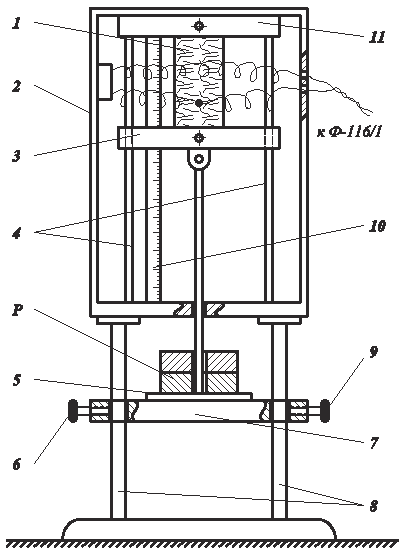
\includegraphics[scale=1]{Ustanovka.pdf}}
		\caption{Схема установки для исследования термических эффектов при упругой деформации резиновой пленки.}
		\label{ris:ustanovka}
	\end{figure}

\section{Модель эксперимента}
	\subsection{Исследвоание зависимости удлинения резины от величины груза, растягивающего образец}
		Исследуем растяжение резины, сняв 7 экспериментальных точек при $1 \leq \lambda \leq 2$ Чтобы обеспечить изотермические условия опыта, будем выжидать не менее двух минут после установки каждого нового груза. Измерения начнем с самого большого груза, т.е. с груза, который растягивает резину примерно в 2 раза.
		
		Построим график расстяжения, откладывая по оси абсцисс силу $f$, а по оси ординат -- выражение $\lambda - 1 / \lambda^2$. Из графика найдём модуль Юнга $E$ для резины.
		
		
	\subsection{Исследование термических эффектов, сопровождающих растяжение резины}
		Исследуем, как меняется температура резины в зависимости от времени. Для этого на осицллограф подадим сигнал с термопары, нагрузим платформу самым большим грузом и быстро опустим его таким образом, чтобы время опускания было мало, а колебания не возникли. Измерения будем проводить в течение нескольких минут, пока не установится тепловое равновесие.
		
		Полученные данные используем для построения зависимости $\ln \Delta T$ от $t$. Аппроксимируя полученный график к моменту $t = 0$, определим величину $\Delta T_0$.
		
		
\section{Экспериментальные данные}
	В таблице~\ref{table:parametri} приведены параметры установки и случайные ошибки измерения величин, определяемых в ходе эксперимента.
	
	\floatsetup[table]{capposition=top}	
	\begin{table}[H]
		\caption{Некоторые параметры установки и ошибки измерений.}
		\label{table:parametri}
\begin{tabular}{|c|c|c|c|c|}
\hline
                  & \begin{tabular}[c]{@{}c@{}}Начальная длина\\ $l_0$, мм\end{tabular} & \begin{tabular}[c]{@{}c@{}}Площадь поперечного сечения\\ $\sigma_0$, см$^2$\end{tabular} & \begin{tabular}[c]{@{}c@{}}Масса\\ $m$, г\end{tabular} & Чувств., В/$^\circ$C \\ \hline
Величина          & 103                                                                 & 0,24                                                                                     & 140                                                    & 0,195                \\ \hline
Погрешность       & 0,5                                                                 & 0                                                                                        & 0,5                                                    & 0                    \\ \hline
$\varepsilon$, \% & 0,5                                                                 & 0                                                                                        & 0,4                                                    & 0                    \\ \hline
\end{tabular}
	\end{table}	

	В следующей таблице представлены результаты измерений, проведенных в первой части лабораторной работы.
	\floatsetup[table]{capposition=top}	
	\begin{table}[H]
		\caption{Результаты измерений и вычислений.}
		\label{table:results_1}
		\begin{tabular}{|c|c|c|c|c|c|c|}
\hline
$m$, кг & $l$, мм & $\lambda$ & $f$, Н & $\lambda - 1/ \lambda^2$ & $E$, МПа             & $\varepsilon_E$, \%   \\ \hline
1,186   & 189     & 1,83      & 11,63  & 1,54                     & \multirow{7}{*}{0,89} & \multirow{7}{*}{1,13} \\ \cline{1-5}
1,007   & 173     & 1,68      & 9,88   & 1,33                     &                      &                       \\ \cline{1-5}
0,829   & 156     & 1,51      & 8,13   & 1,08                     &                      &                       \\ \cline{1-5}
0,654   & 142     & 1,38      & 6,42   & 0,85                     &                      &                       \\ \cline{1-5}
0,477   & 127     & 1,23      & 4,68   & 0,58                     &                      &                       \\ \cline{1-5}
0,351   & 119     & 1,16      & 3,44   & 0,41                     &                      &                       \\ \cline{1-5}
0,174   & 109     & 1,06      & 1,71   & 0,17                     &                      &                       \\ \hline
\end{tabular}
	\end{table}
	На рис.~\ref{ris:Graph_1} изображен график зависимости $\lambda - 1/ \lambda^2$ от $f$ в изотермическом процессе.
	
	\begin{figure}[H]
		\center{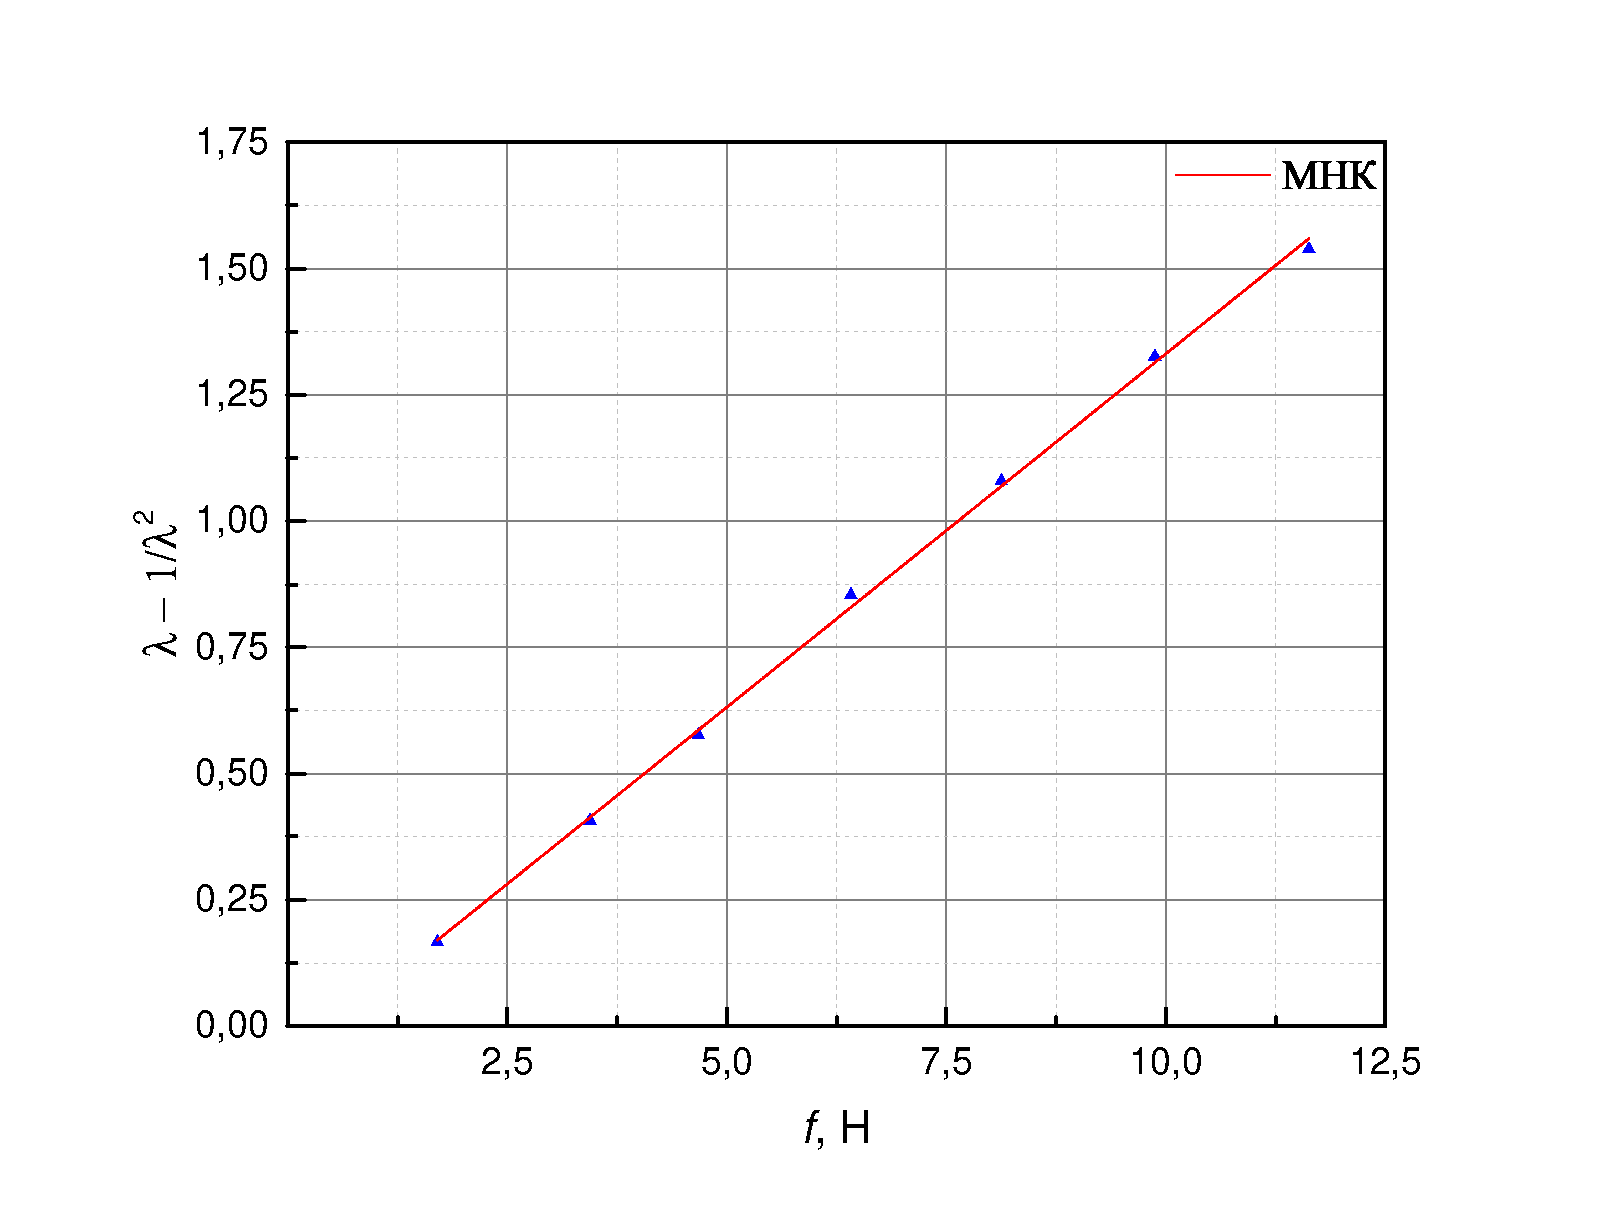
\includegraphics[scale=0.5]{Graph_1.pdf}}
		\caption{Зависимость $\lambda - 1/ \lambda^2$ от $f$.}
		\label{ris:Graph_1}
	\end{figure}

\newpage
\thisfloatsetup{floatrowsep=mysep}	
\begin{figure}[h!]
\begin{floatrow}
 \ffigbox[\FBwidth]{\caption{Зави-ть $\ln V$ от $t$ ($m = 1,186$ кг).}\label{fig:Graph_2_1}}%
         {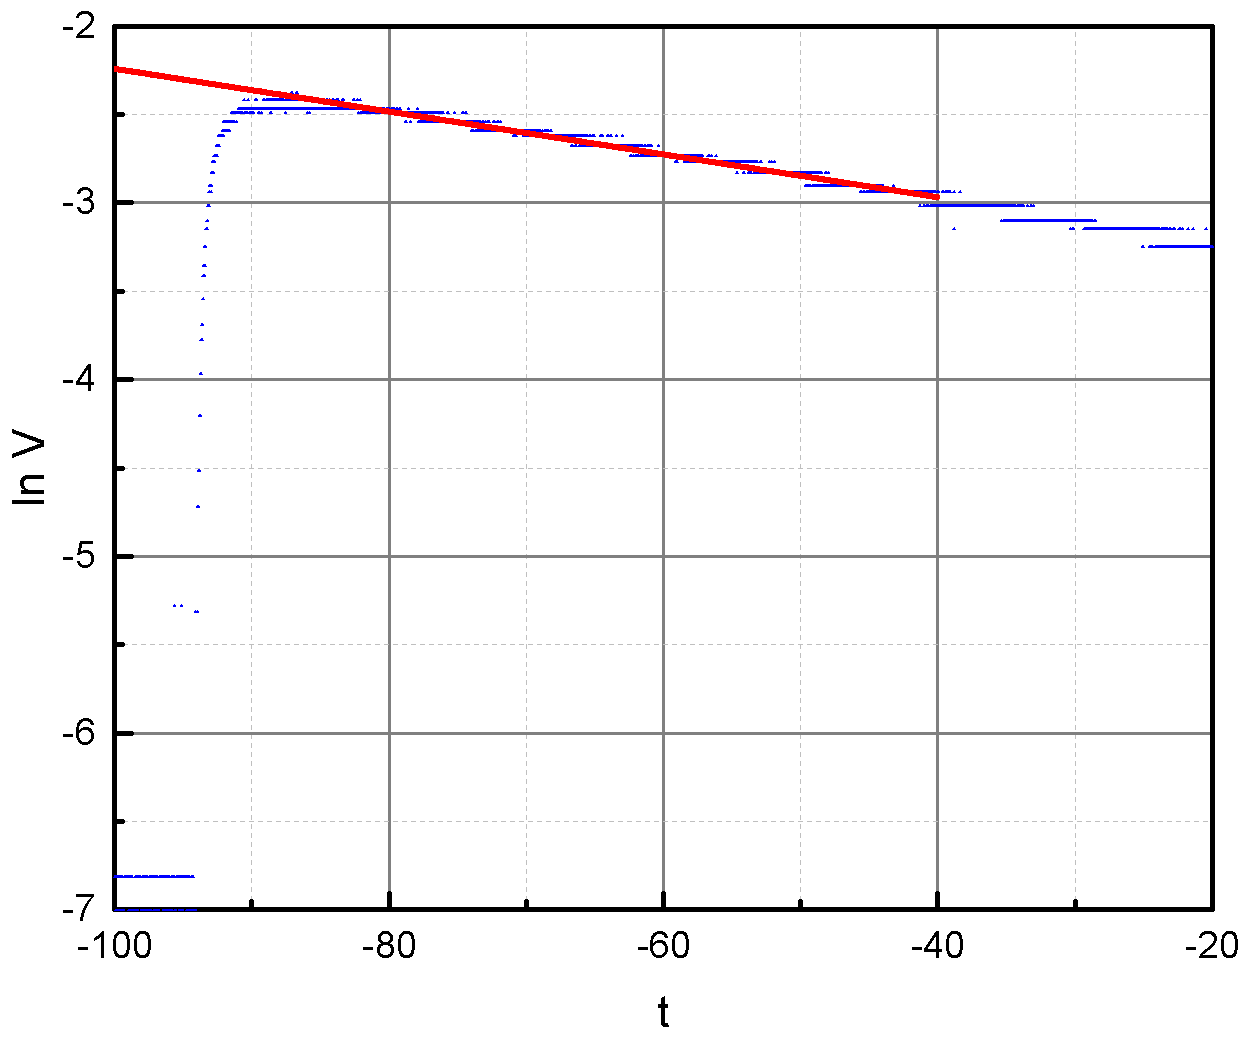
\includegraphics[width=8cm,height=7cm]{Graph_2_1}}
 \ffigbox[\FBwidth]{\caption{Зави-ть $\ln V$ от $t$ ($m = 1,007$ кг).}\label{fig:Graph_2_2}}%
         {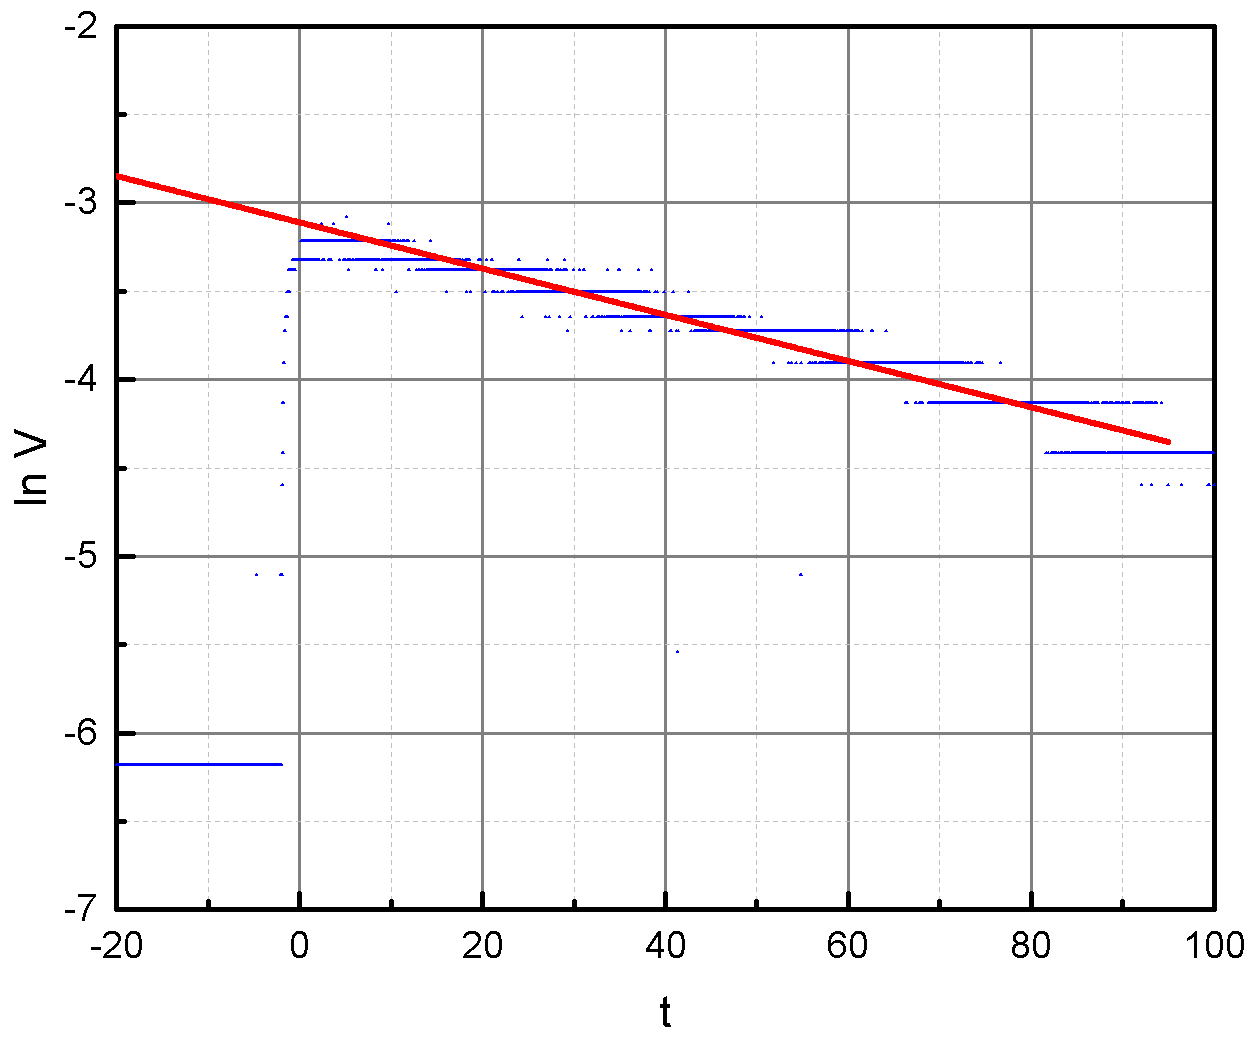
\includegraphics[width=8cm,height=7cm]{Graph_2_2}}         
\end{floatrow}
\end{figure}

\thisfloatsetup{floatrowsep=mysep}	
\begin{figure}[h!]
\begin{floatrow}
 \ffigbox[\FBwidth]{\caption{Зави-ть $\ln V$ от $t$ ($m = 0,829$ кг).}\label{fig:Graph_2_3}}%
         {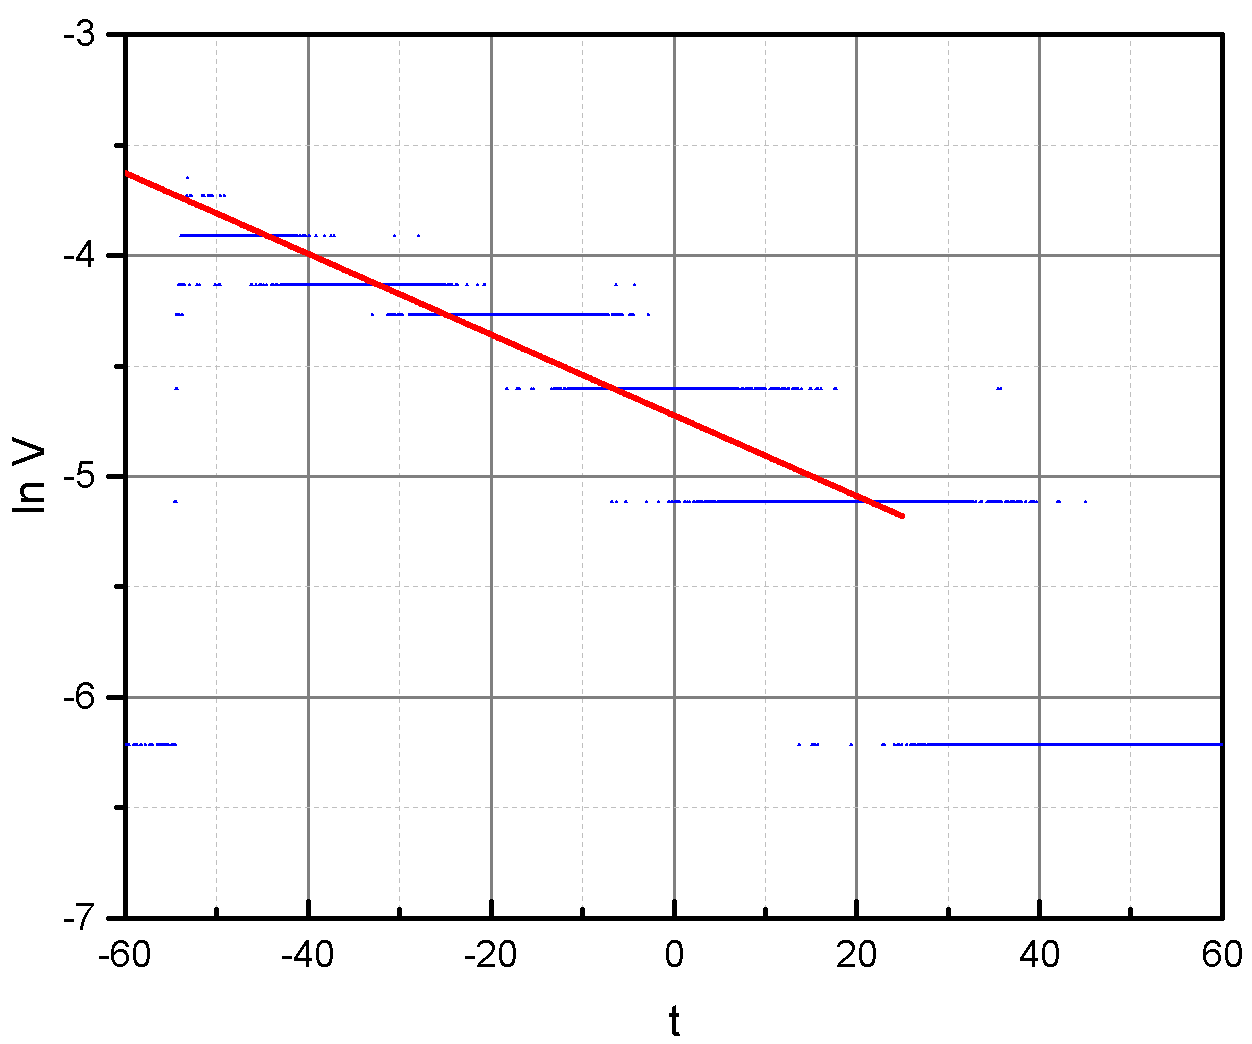
\includegraphics[width=8cm,height=7cm]{Graph_2_3}}
 \ffigbox[\FBwidth]{\caption{Зави-ть $\ln V$ от $t$ ($m = 0,654$ кг).}\label{fig:Graph_2_4}}%
         {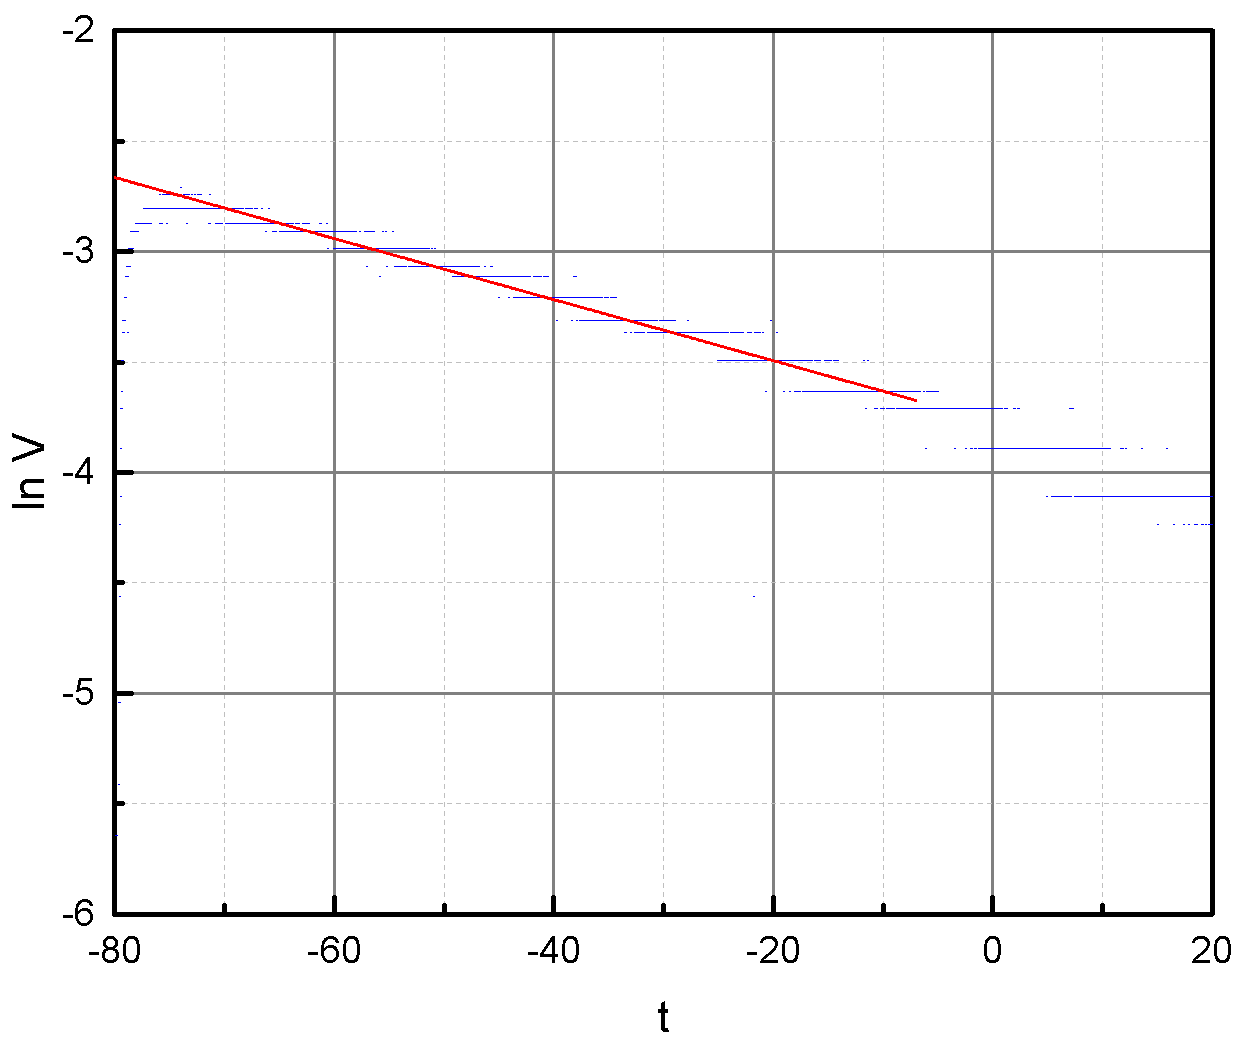
\includegraphics[width=8cm,height=7cm]{Graph_2_4}}         
\end{floatrow}
\end{figure}

	\floatsetup[table]{capposition=top}	
	\begin{table}[H]
		\caption{Результаты вычислений.}
		\label{table:results_2}
		\begin{tabular}{|c|c|c|}
\hline
$m$, кг & $\Delta T_0$, К & $C_l$, Дж/К \\ \hline
1,186   & 0,510          & 1,038 \\ \hline
1,007   & 0,363          & 1,011 \\ \hline
0,829   & 0,236          & 0,939 \\ \hline
0,654   & 0,137          & 0,918 \\ \hline
\end{tabular}
	\end{table}



\section{Обсуждение результатов}
	Итак, в ходе данной лабораторной работы мы убедились в термических свойствах деформации резины ($1,3 \leq \lambda \leq 2$): при растяжении она нагревается, а не охлаждается, как большинство упругих тел. Экспериментально установили, что силы упругости в резине при постоянной температуре ($T = 20^\circ$C) удовлетворяют следующему соотношению $f \propto \lambda - 1 / \lambda^2$. Вычислили модуль Юнга $E = (0,89 \pm 0,01)$ МПа. Теплоемкость резины при постоянной длине возьмем при $m = 1,186$ $C_l = 1,038$ Дж/К, так как при этой массе растяжение наибольшое и изменение температуры наибольшое, следовательно, погрешность измерения будет минимальной. Более того, в реальных экспериментальных условиях растяжение резины не является строго адиабатическим. Вследствие теплоотвода (необратимости) измеренное значение $\Delta T$ оказывается меньше теоретического.
	
	Тепловые эффекты деформации очень важно изучать, так как они могут отрицательно сказываться на структуре и свойствах резиновых изделий.
	
\section{Выводы}
\begin{enumerate}
	\item
		Установили, что в изотермическом процессе $f \propto \lambda - 1 / \lambda^2$.
	\item
		Вычислили модуль Юнга для исследуемого резиного материала $E = (0,89 \pm 0,01)$ МПа.
	\item
		Определили теплоёмкость материала при постоянной длине $C_l = 1,038$ Дж/К.
		
\end{enumerate}



























\end{document}